\documentclass[11pt,letterpaper]{article}

\usepackage[utf8]{inputenc}
\usepackage[spanish]{babel}
\usepackage{graphicx}
\usepackage{float}
\usepackage{geometry}
\geometry{top=2.5cm, bottom=2.5cm, left=2.5cm, right=2.5cm}

\usepackage{listings}
\usepackage{color}
\usepackage{longtable}

\definecolor{keyblue}{rgb}{0,0,0.6}
\definecolor{strgreen}{rgb}{0,0.5,0}
\definecolor{graycomments}{rgb}{0.5,0.5,0.5}

\lstset{
    language=SQL,
    basicstyle=\ttfamily\small,
    keywordstyle=\color{keyblue}\bfseries,
    stringstyle=\color{strgreen},
    commentstyle=\color{graycomments}\itshape,
    breaklines=true,
    showstringspaces=false
}

\author{Christian González de León}
\title{Análisis de ingeniería inversa sobre un sistema \textit{Legacy}}
\date{\today}

\begin{document}
\maketitle

\begin{abstract}
Esta es la documentación del análisis de la base de datos ``Escuela'' aplicándole ingeniería inversa.
\end{abstract}

\section{Introducción}
La instrucción de esta actividad es analizar 2 scripts, el primero es la estructura de la base de datos y el segundo es para insertar los datos en la base de datos y así poder hacer el análisis mediante MySQL Workbench aplicándole ingeniería inversa.

\section{Descripción del problema}
El sistema escolar cuenta con un diseño de base de datos relacional operativo, pero carece de documentación activa y de consultas estandarizadas para obtener reportes básicos. Esto impide que la institución pueda monitorear de forma rápida el desempeño de los alumnos, la carga de trabajo de los profesores y la disponibilidad de los salones. El problema consiste en analizar el esquema existente mediante ingeniería inversa para diseñar y validar las consultas SQL necesarias que resuelvan estas necesidades de información.

\section{Análisis}
A partir de las consultas ejecutadas en MySQL Workbench, se comprobó que el modelo relacional de la escuela funciona de manera correcta y respeta las reglas del negocio.

Por un lado, las instrucciones JOIN demostraron que las tablas maestras están bien conectadas con sus llaves primarias y foráneas, permitiendo cruzar datos complejos como los salones, horarios y las calificaciones de los alumnos sin errores.

Por otro lado, el uso de LEFT JOIN sirvió para identificar casos especiales, como el curso de Etica que aparece correctamente en el sistema a pesar de tener cero estudiantes inscritos.

Finalmente, las consultas con GROUP BY y HAVING confirmaron que la planta docente está equilibrada con un profesor por departamento, ayudando también a detectar rápido a los alumnos con alta carga de materias y los promedios más bajos para tomar decisiones escolares.
\subsection{Preguntas}
Preguntas que se deben responder en base al esquema de base de datos 'escuela'\\

\begin{enumerate}
    \item \textbf{¿Cuáles son los estudiantes inscritos en el curso Álgebra?}
    
    Dos alumnos son los que están inscritos: Juan Pérez y María Gómez.
\begin{lstlisting}
SELECT e.nombre, e.apellido 
FROM estudiantes e
JOIN inscripciones i ON e.id = i.id_estudiante
JOIN cursos c ON i.id_curso = c.id
WHERE c.nombre = 'Algebra';
\end{lstlisting}

    \item \textbf{¿Qué cursos imparte el profesor Pedro Martínez?}
    
    El curso de 'Programación' que vale 6 créditos.
\begin{lstlisting}
SELECT c.nombre AS curso, c.creditos 
FROM cursos c
JOIN profesores p ON c.id_profesor = p.id
WHERE p.nombre = 'Pedro' AND p.apellido = 'Martinez';
\end{lstlisting}

    \item \textbf{¿Cuántos estudiantes están inscritos en cada curso?}
    
    En Álgebra están inscritos 2, Biología 1, Historia 1, Programación 1, Física 1 y Ética 0.
\begin{lstlisting}
SELECT c.nombre AS curso, COUNT(i.id_estudiante) AS total_estudiantes
FROM cursos c
LEFT JOIN inscripciones i ON c.id = i.id_curso
GROUP BY c.id, c.nombre;
\end{lstlisting}

    \item \textbf{¿Cuál es el promedio de notas por curso?}
    
    El promedio de notas en Álgebra es 8, Biología 9, Historia 6.8, Programación 9.2, y Física 7.
\begin{lstlisting}
SELECT c.nombre AS curso, ROUND(AVG(n.nota), 2) AS promedio_notas
FROM cursos c
JOIN inscripciones i ON c.id = i.id_curso
JOIN notas n ON i.id = n.id_inscripcion
GROUP BY c.id, c.nombre;
\end{lstlisting}

    \item \textbf{Lista de estudiantes con notas mayores a 8.0}
    
    El alumno con la nota más alta bajo este límite es Carlos Sánchez con 9.2, luego Juan Pérez con 2 notas: 9 y 8.5.
\begin{lstlisting}
SELECT DISTINCT e.nombre, e.apellido, n.nota
FROM estudiantes e
JOIN inscripciones i ON e.id = i.id_estudiante
JOIN notas n ON i.id = n.id_inscripcion
WHERE n.nota > 8.0;
\end{lstlisting}

    \item \textbf{¿Qué cursos tienen más de una inscripción?}
    
    El curso de Álgebra es el que tiene 2 inscripciones.
\begin{lstlisting}
SELECT c.nombre AS curso, COUNT(i.id) AS total_inscripciones
FROM cursos c
JOIN inscripciones i ON c.id = i.id_curso
GROUP BY c.id, c.nombre
HAVING COUNT(i.id) > 1;;
\end{lstlisting}

    \item \textbf{¿Qué profesores pertenecen al departamento de 'Ingeniería'?}
    
    Solo el profesor Pedro Martínez es el que pertenece al departamento.
\begin{lstlisting}
SELECT p.nombre, p.apellido, p.email 
FROM profesores p
JOIN departamentos d ON p.id_departamento = d.id
WHERE d.nombre = 'Ingenieria';
\end{lstlisting}

    \item \textbf{¿Cuáles son los cursos programados los lunes?}
    
    La única clase programada para los lunes es la clase de Álgebra de 8 a 10.
\begin{lstlisting}
SELECT DISTINCT c.nombre AS curso, h.hora_inicio, h.hora_fin
FROM cursos c
JOIN horarios h ON c.id = h.id_curso
WHERE h.dia_semana = 'Lunes';
\end{lstlisting}

    \item \textbf{¿Qué aulas tienen una capacidad mayor a 25?}
    
    La sala de conferencias y el Aula 101 son las aulas con más capacidad, contando con 50 y 30 personas de capacidad respectivamente.
\begin{lstlisting}
SELECT nombre AS aula, capacidad 
FROM aulas
WHERE capacidad > 25;
\end{lstlisting}

    \item \textbf{Lista de cursos con su aula y horario}
    
    Álgebra - Aula 101 - Lunes de 8:00am - 10:00am\\
    Biología - Aula 102 - Martes de 10:00am - 12:00am\\
    Física - Aula 102 - Viernes de 8:00am - 10:00am\\
    Programación - Laboratorio 1 - Jueves de 9:00am - 11:00am\\
    Historia - Sala de conferencias - Miércoles de 13:00pm - 15:00pm
\begin{lstlisting}
SELECT c.nombre AS curso, a.nombre AS aula, h.dia_semana, h.hora_inicio, h.hora_fin
FROM cursos c
JOIN horarios h ON c.id = h.id_curso
JOIN aulas a ON h.id_aula = a.id;
\end{lstlisting}

    \item \textbf{¿Qué estudiantes tiene la nota más alta y en qué cursos?}
    
    Carlos Sánchez en Programación con una nota de 9.2.
\begin{lstlisting}
SELECT e.nombre, e.apellido, c.nombre AS curso, n.nota
FROM estudiantes e
JOIN inscripciones i ON e.id = i.id_estudiante
JOIN cursos c ON i.id_curso = c.id
JOIN notas n ON i.id = n.id_inscripcion
WHERE n.nota = (SELECT MAX(nota) FROM notas);
\end{lstlisting}

    \item \textbf{¿Cuántos profesores hay por departamento?}
    
    Hay un profesor por departamento.
\begin{lstlisting}
SELECT d.nombre AS departamento, COUNT(p.id) AS cantidad
FROM departamentos d
LEFT JOIN profesores p ON d.id = p.id_departamento
GROUP BY d.id;
\end{lstlisting}

    \item \textbf{¿Qué cursos no tienen estudiantes inscritos?}
    
    Ética es el curso que no tiene ningún estudiante.
\begin{lstlisting}
SELECT c.nombre AS curso_vacio
FROM cursos c
LEFT JOIN inscripciones i ON c.id = i.id_curso
WHERE i.id_estudiante IS NULL;
\end{lstlisting}

    \item \textbf{¿Qué estudiantes están inscritos en más de un curso?}
    
    Juan Pérez y María Gómez están inscritos a 2 cursos cada uno.
\begin{lstlisting}
SELECT e.nombre, e.apellido, COUNT(i.id_curso) AS total_cursos
FROM estudiantes e
JOIN inscripciones i ON e.id = i.id_estudiante
GROUP BY e.id, e.nombre, e.apellido
HAVING COUNT(i.id_curso) > 1;
\end{lstlisting}

    \item \textbf{¿Cuál es el curso con menor promedio de notas?}
    
    Historia con un promedio de 6.8.
\begin{lstlisting}
SELECT c.nombre AS curso, ROUND(AVG(n.nota), 2) AS promedio_mas_bajo
FROM cursos c
JOIN inscripciones i ON c.id = i.id_curso
JOIN notas n ON i.id = n.id_inscripcion
GROUP BY c.id, c.nombre
ORDER BY promedio_mas_bajo ASC
LIMIT 1;
\end{lstlisting}
\end{enumerate}

\section{Diagramas}

En esta sección se muestra el modelo relacional recuperado mediante el proceso de ingeniería inversa en la herramienta MySQL Workbench

\begin{figure}[H]
    \centering
    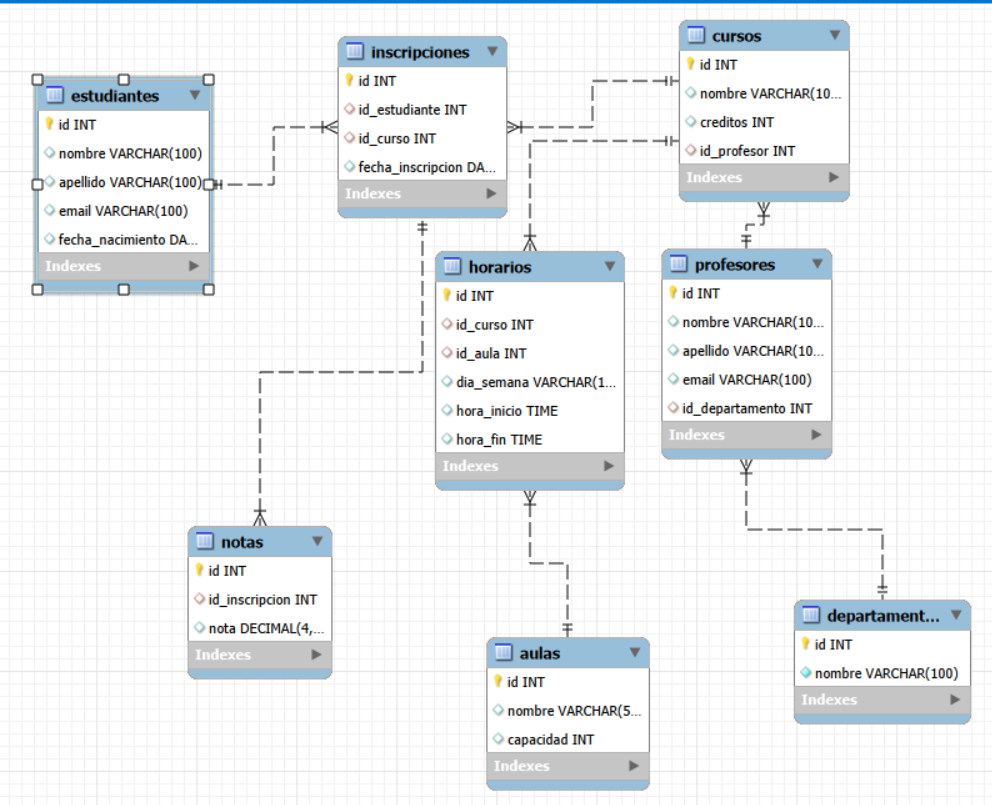
\includegraphics[width=0.7\textwidth]{Diagrama.png}
    \caption{Diagrama Entidad-Relacion (DER) obtenido en MySQL Workbench}
\end{figure}


\section{Conclusiones}
Como conclusión, la aplicación de ingeniería inversa sobre la base de datos de la escuela permitió entender a fondo cómo está estructurado el sistema y recuperar toda su lógica de funcionamiento. Al meter datos de prueba y ejecutar las quince consultas, se demostró que las tablas están perfectamente conectadas entre sí y que las reglas escolares se cumplen sin errores. Este tipo de análisis es muy útil en el mundo real para ordenar y sacar reportes limpios de cualquier base de datos que no tenga manuales ni documentación previa.

\end{document}